\section{1174008 - Arjun Yuda Firwanda}
\subsection{Teori}
\begin{enumerate}
	\item Definisi Kecerdasan Buatan
	\hfill\break
	Definisi Kecerdasan Buatan (Artificial Intelligence) yakni sebagai kecerdasan entitas ilmiah. Kecerdasan Buatan diciptakan dalam suatu mesin komputer agar dapat melakukan pekerjaan seperti halnya yang dilakukan manusia.
	
	\item Sejarah dan Perkembangan Kecerdasan Buatan
	\hfill\break
	Sejarah dan Kecerdasan Buatan tidak lepas dari sosok John McCarthy. Ia sebagai "Bapak AI".

	\begin{itemize}
		\item Cikal bakal kecerdasan buatan (tahun 1943 - 1955)
		
		\item Kelahiran Kecerdasan Buatan (tahun 1956)
		
		\item Awal kecerdasan buatan merupakan tahap pengembangan aplikasi AI yang sukses dibandingkan dengan program komputer (tahun 1952 - 1969)
		
		\item Kecerdasan Buatan menjadi industry  (tahun 1980 - sekarang)
		
		\item Kecerdasan Buatan menjadi disiplin ilmu (tahun 1987 - sekarang)
		
		\item Kecerdasan Buatan menampakkan diri di semua bidang (tahun 1995 - sekarang)

	\end{itemize}

	\item Definisi Supervised Learning
	\hfill\break
	Supervised Learning merupakan pembelajaran yang ada supervisornya. Maksudnya adalah label di tiap data nya. Label maksudnya merupakan sebuatan tag dari data yang ditambahkan dalam machine learning model.
	
	\item Regresi
	\hfill\break
	Regresi merupakan menebak nilai output dari nilai input yang diberikan, berdasarkan pola input - ouput sebelumnya.

	\item Klasifikasi
	\hfill\break
	Klasifikasi, merupakan mengetahui jenis kelamin siswa dari tinggi dan berat badannya.

	\item Definisi Unsupervised Learning
	\hfill\break
	Unsupervised learning memiliki keunggulan. Jika unsupervised learning memiliki label sebagai dasar prediksi baik serta membuat clasification dan regression algorithm K-Means, Hierarchical Clustering, DBSCAN, Fuzzy C-Means, Self-Organizing Map.

	\item Data Set
	\hfill\break
	Data Set, merupakan objek yang merepresentasikan data dan relasinya. Strukturnya mirip dengan data di database. Dataset berisi koleksi dari datatable dan datarelation.

	\item Trainning Set
	\hfill\break
	Trainning Set, merupakan konteks machine learning Training = latihan.

	\item Testing Set
	\hfill\break
	Testing Set, merupakan melakukan evaluasi terhadap performa algoritma tersebut. Pada proses testing ini, dilakukan untuk mwengetahui performa algoritma akan diuji menggunakan testing set, dimana testing set dan training set merupakan data yang berbeda.

\end{enumerate}


\subsection{Praktek}
\begin{enumerate}
	\item Instalasi Library scikit dari ianaconda, mencoba kompilasi dan uji coba ambil contoh kode dan lihat variabel explorer
	\hfill\break
	\begin{figure}[H]
		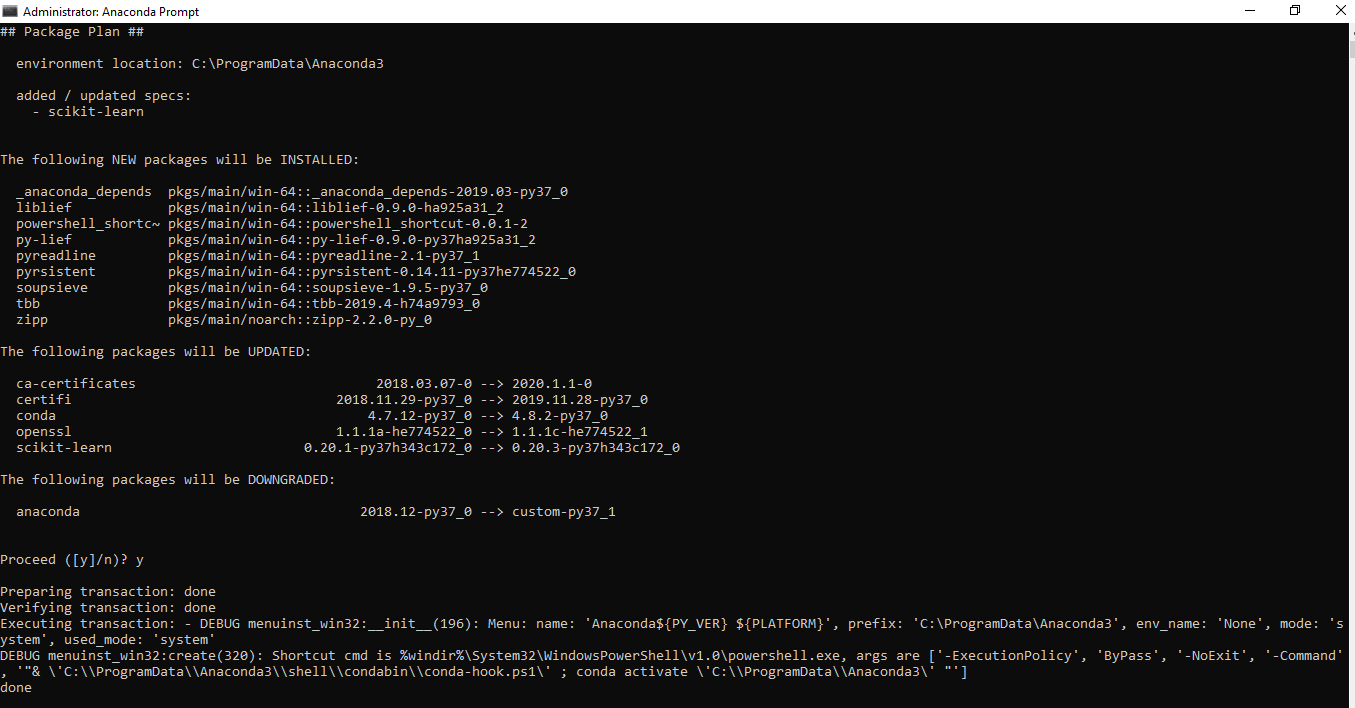
\includegraphics[width=4cm]{figures/1174008/1/instalasi.PNG}
		\centering
		\caption{Instalasi Package Scikit Learn}
	\end{figure}
	\begin{figure}[H]
		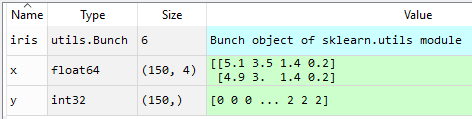
\includegraphics[width=4cm]{figures/1174008/1/variable.PNG}
		\centering
		\caption{Isi Variabel Explorer}
	\end{figure}

	\item Mencoba loading an example dataset
	\hfill\break
	\lstinputlisting[firstline=7, lastline=11]{src/1174008/1/1174008.py}

	\item Mencoba Learning dan predicting
	\hfill\break
	\lstinputlisting[firstline=13, lastline=22]{src/1174008/1/1174008.py}

	\item Mencoba Model Persistence
	\hfill\break
	\lstinputlisting[firstline=25, lastline=34]{src/1174008/1/1174008.py}

	\item Mencoba Conventions
	\hfill\break
	\lstinputlisting[firstline=37, lastline=48]{src/1174008/1/1174008.py}
\end{enumerate}

\subsection{Penanganan Error}
\begin{enumerate}
	\item ScreenShoot Error
	\begin{figure}[H]
		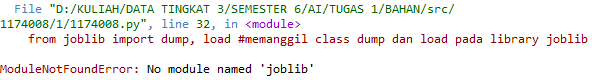
\includegraphics[width=4cm]{figures/1174008/error/error.PNG}
		\centering
		\caption{ Error Joblib}
	\end{figure}

	\item Tuliskan Kode Error dan Jenis Error
	\begin{itemize}
		\item Import Error
		\item Value Error
	\end{itemize}

	\item Cara Penangan Error
	\begin{itemize}
		\item Import Error
		\hfill\break
		Dengan Menginstall Library Yang Tidak Ditemukan
		\item Value Error
		\hfill\break
		Mengubah Bentuk Arraynya, Menjadi 1 Dimensi
	\end{itemize}
\end{enumerate}

\subsection{Bukti Tidak Plagiat}
\begin{figure}[H]
	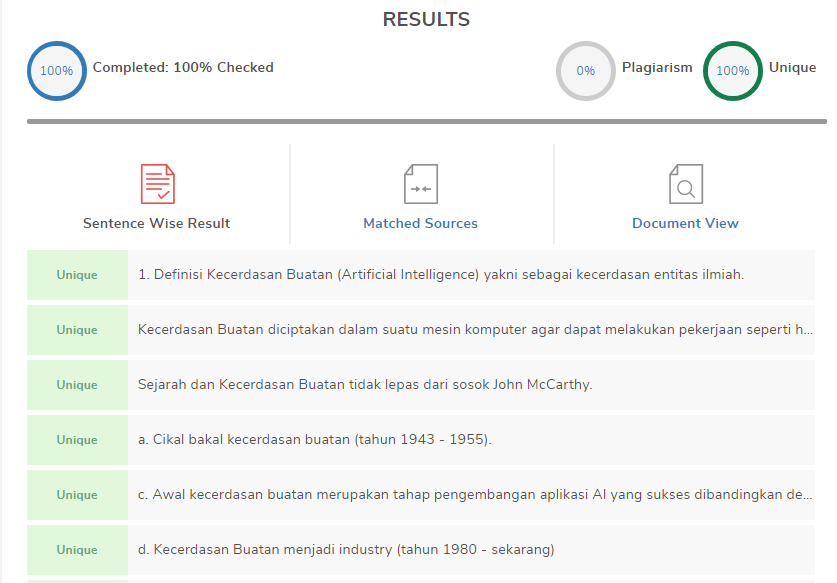
\includegraphics[width=4cm]{figures/1174008/bukti/CekPlagiarisme.PNG}
	\centering
	\caption{Bukti Tidak Melakukan Plagiat Chapter 1}
\end{figure}